\documentclass{beamer}

\usepackage[utf8]{inputenc}
\usecolortheme{beaver}
\usepackage{caption}
\usepackage{subcaption}

\setbeamertemplate{footline}[text line]{%
  \parbox{\linewidth}{\vspace*{-8pt} Kuroki, M., \& Pearl, J. (2014). Measurement bias and effect restoration in causal inference \hfill\insertshortauthor\hfill\insertpagenumber}}
\setbeamertemplate{navigation symbols}{}

\begin{document}

\begin{frame}
\frametitle{Problem Statement}

\begin{center}
Identification: Can the causal effect of $ X $ on $ Y $ be uniquely estimated given the distribution and model structure?
\end{center}

\begin{figure}
    \centering
    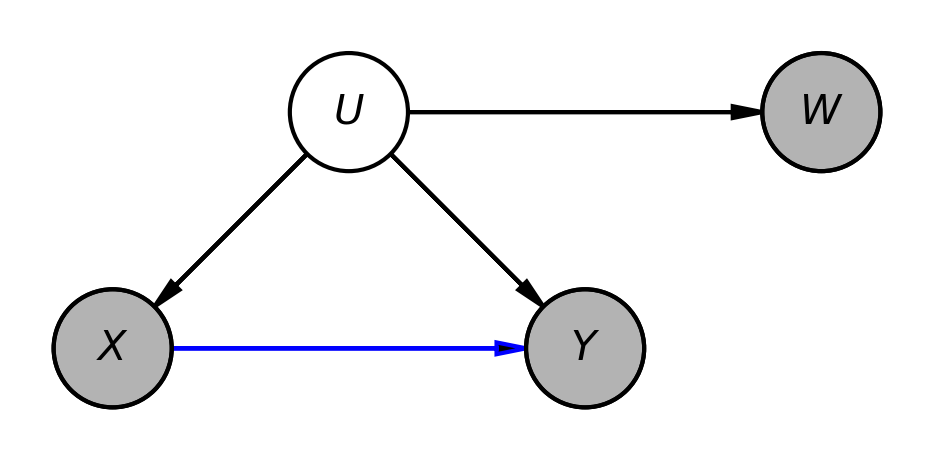
\includegraphics[scale=0.6]{scripts/single_proxy.png}
    \label{fig:non_iden}
\end{figure}

\begin{center}
	$ pr\{y | do(x)\} = \sum_{u} pr(y | x, u) pr(u) $ 
\end{center}
\end{frame}

\begin{frame}
\frametitle{Case 1: Single proxy variable with known error mechanism}

\begin{columns}
\column{0.5\textwidth}
	Required: $ pr(w | u) $
	
	\bigskip

	Use matrix adjustment to estimate $ pr(y | x, u) $ and $ pr(u) $.

\column{0.5\textwidth}

    \begin{figure}
    	\centering
    	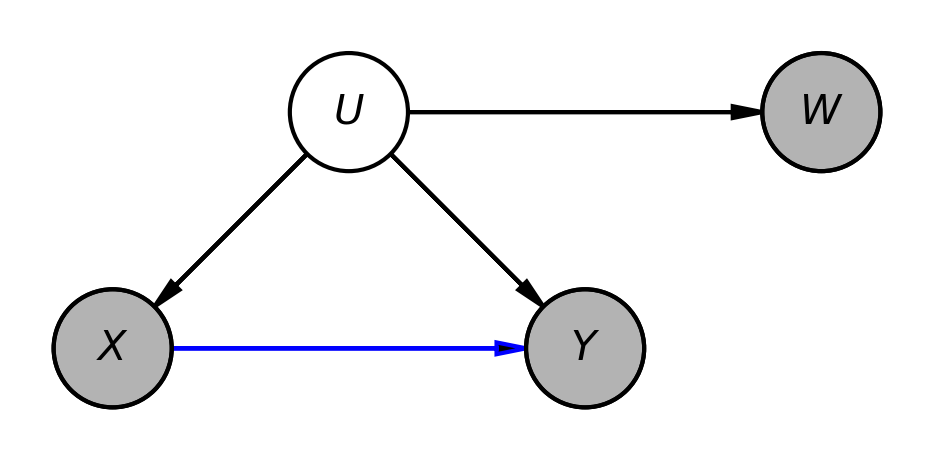
\includegraphics[scale=0.6]{scripts/single_proxy.png}
    \end{figure}

\end{columns}

\end{frame}

\begin{frame}
\frametitle{Case 2: Multiple proxy variables.}
\begin{columns}
\column{0.5\textwidth}
	Required: One proxy variable should only be connected to $ U $.

	\bigskip

	\begin{enumerate}
		\item Choose one of the proxy variables as the ``indicator variable'', $ W $.
		\item Use eigen value decomposition to estimate $ pr(w | u) $.
		\item Follow the method of first case.
	\end{enumerate}

\column{0.5\textwidth}

    \begin{figure}
	\begin{subfigure}{0.5\textwidth}
    		\centering
    		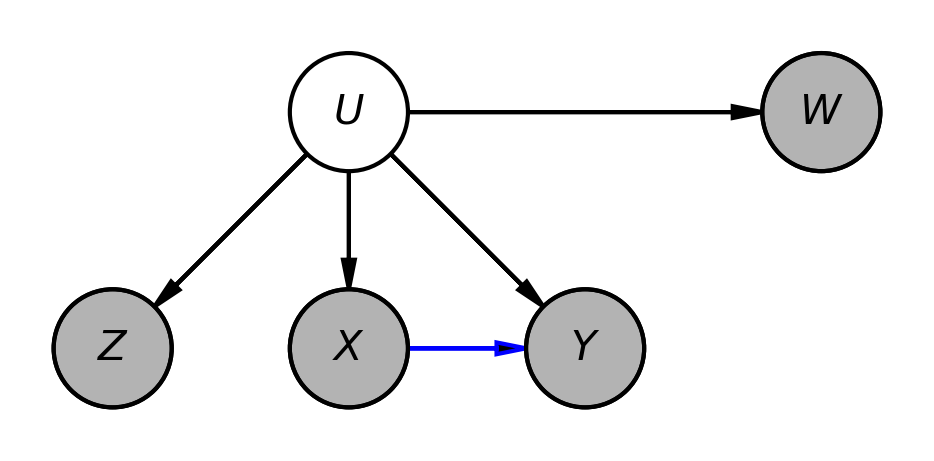
\includegraphics[scale=0.6]{scripts/double_proxy.png}
	\end{subfigure}
	\begin{subfigure}{0.5\textwidth}
    		\centering
    		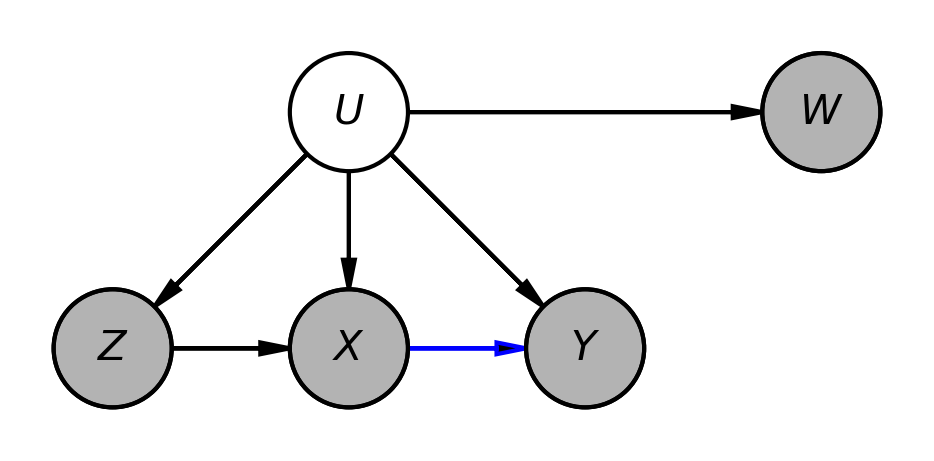
\includegraphics[scale=0.6]{scripts/double_proxy_with_extra_edge.png}
	\end{subfigure}
    \end{figure}

\end{columns}

\end{frame}

\begin{frame}
\frametitle{Case 3: Linear SEM}

\begin{columns}
\column{0.5\textwidth}

	Required: The contribution of $U$'s variance to $W$'s variance: $ \alpha_{wu}^2 \sigma_{uu} = \sigma_{ww} - \sigma_{\epsilon_w, \epsilon_w} $

	\bigskip

	\begin{enumerate}
		\item If single proxy variable, needs $ \alpha_{wu}^2 \sigma_{uu} $.
		\item If multiple proxy variables, $ \alpha_{wu}^2 \sigma_{uu} $ can be computed.
	\end{enumerate}

\column{0.5\textwidth}
	\begin{figure}
    		\centering
    		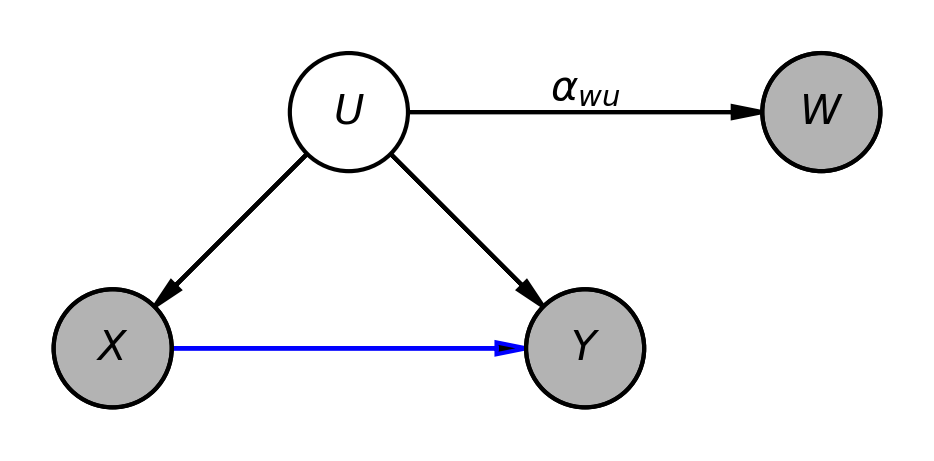
\includegraphics[scale=0.6]{scripts/sem.png}
	\end{figure}
\end{columns}

\end{frame}

\begin{frame}
\frametitle{Case 4: Linear SEM with instrumental variables}

    \begin{figure}
    	\centering
    	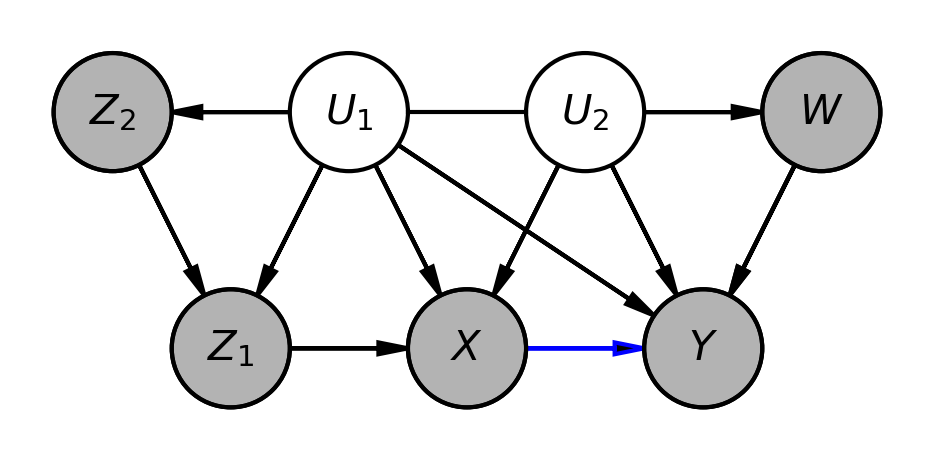
\includegraphics[scale=0.6]{scripts/instrumental_var.png}
    \end{figure}

    \begin{figure}
    	\centering
    	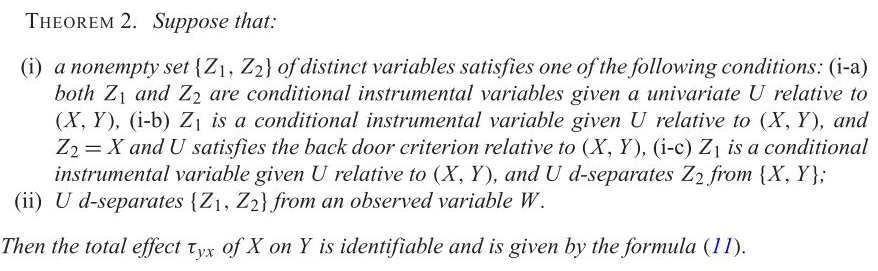
\includegraphics[scale=0.6]{scripts/theorem.png}
    \end{figure}



\end{frame}

\end{document}
